% AY2014 制御工学 解答例
% 回答の流れ・言葉遣いは 03_制御工学/参考/「制御工学Ⅱ（完成版）」に寄せる。
% デザイン（囲み枠等）は真似しない。解答・数値は本年度過去問から自力で導いた。
\documentclass[11pt,a4paper]{article}
\usepackage{../../../00_common/preamble}

\usetikzlibrary{positioning,arrows.meta,calc}
\usepackage{pgfplots}
\pgfplotsset{compat=newest}

\title{制御工学 AY2014 解答例（専門応用科目I）}
\author{}
\date{}

\begin{document}
\maketitle

% ==================================================================
\section*{第1問}

二次振動系（質量 $m$、粘性係数 $d$、バネ定数 $k$）。運動方程式は $m\ddot{x}+d\dot{x}+kx=f(t)$。

\subsection*{(1) 伝達関数・固有振動数・減衰係数}
初期値ゼロでラプラス変換して
\begin{align*}
  &\qquad (ms^2+ds+k)\,X(s)=F(s)
   \quad\therefore\quad G(s)=\frac{1}{ms^2+ds+k}.
\end{align*}
標準形 $\dfrac{1/m}{s^2+2\zeta\omega_n s+\omega_n^2}$ と係数比較して $\omega_n^2=\dfrac{k}{m}$、$2\zeta\omega_n=\dfrac{d}{m}$。
\[
  \therefore\quad \ans{\;G(s)=\dfrac{1}{ms^2+ds+k}\;},\quad
  \ans{\;\omega_n=\sqrt{\dfrac{k}{m}}\;},\quad
  \ans{\;\zeta=\dfrac{d}{2\sqrt{km}}\;}
\]

\subsection*{(2) 定常値が $5$ になる $\beta$}
$m=1$, $d=1$, $k=\beta$、単位ステップ入力。安定なら零入力応答は減衰し、初期値によらず
定常値は強制応答で決まる。最終値の定理より
\begin{align*}
  &\qquad x(\infty)=\lim_{s\to0}\frac{1}{s^2+s+\beta}=\frac{1}{\beta}\\
  &\therefore\quad \frac{1}{\beta}=5.
\end{align*}
\[
  \therefore\quad \ans{\;\beta=\dfrac15\;}
\]

\subsection*{(3) ステップ応答（$m=1,d=3,k=2$、$x(0)=5,\dot x(0)=-1$）}
方程式は $\ddot{x}+3\dot{x}+2x=1$。特性根は $s^2+3s+2=(s+1)(s+2)=0$ より $s=-1,-2$。
特解 $x_p=\tfrac12$ を加えて $x(t)=\tfrac12+A\e^{-t}+B\e^{-2t}$ とおき、初期条件を入れる。
\begin{align*}
  &\qquad x(0)=\tfrac12+A+B=5,\qquad \dot{x}(0)=-A-2B=-1\\
  &\therefore\quad A+B=\tfrac92,\quad A+2B=1
   \quad\therefore\quad A=8,\ B=-\tfrac72.
\end{align*}
\[
  \therefore\quad \ans{\;x(t)=\dfrac12+8\e^{-t}-\dfrac72\e^{-2t}\;}
\]
$\dot{x}(t)=\e^{-2t}(7-8\e^{t})<0\ (t>0)$ より単調減少で、$x$ は $5$ から定常値 $\tfrac12$ へ向かう。

\begin{center}
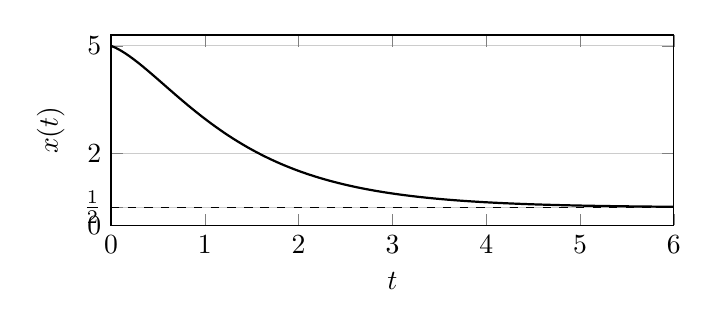
\begin{tikzpicture}
\begin{axis}[
  width=0.72\linewidth, height=4cm,
  xmin=0, xmax=6, ymin=0, ymax=5.3,
  xlabel={$t$}, ylabel={$x(t)$},
  ytick={0,0.5,2,5}, yticklabels={$0$,$\frac12$,$2$,$5$},
  ymajorgrids=true, grid style={gray!40},
]
\addplot[thick,domain=0:6,samples=120]{0.5+8*exp(-x)-3.5*exp(-2*x)};
\addplot[dashed,domain=0:6]{0.5};
\end{axis}
\end{tikzpicture}
\end{center}

\subsection*{(4) 正弦入力応答（$m=1,d=1,k=1$、零初期値、$f(t)=\sin\omega t$）}
$G(s)=\dfrac{1}{s^2+s+1}$、$F(s)=\dfrac{\omega}{s^2+\omega^2}$。$\Delta\equiv\omega^4-\omega^2+1$ とおき、
$X(s)=G(s)F(s)$ を部分分数分解して逆変換する。特性根は $s=-\tfrac12\pm\tfrac{\sqrt3}{2}j$ なので
\begin{align*}
  x(t)&=\underbrace{\frac{\omega}{\Delta}\,\e^{-t/2}\!\left(\cos\tfrac{\sqrt3}{2}t+\tfrac{2\omega^2-1}{\sqrt3}\sin\tfrac{\sqrt3}{2}t\right)}_{\text{過渡項（減衰）}}
   \;-\;\underbrace{\frac{1}{\Delta}\bigl(\omega\cos\omega t+(\omega^2-1)\sin\omega t\bigr)}_{\text{定常項}}.
\end{align*}
定常項は振幅 $\dfrac{\sqrt{\omega^2+(\omega^2-1)^2}}{\Delta}=\dfrac{1}{\sqrt{\Delta}}=|G(j\omega)|$ の正弦波である。
\[
  \therefore\quad \ans{\;x(t)=\dfrac{\omega}{\Delta}\e^{-t/2}\!\left(\cos\tfrac{\sqrt3}{2}t+\tfrac{2\omega^2-1}{\sqrt3}\sin\tfrac{\sqrt3}{2}t\right)-\dfrac{\omega\cos\omega t+(\omega^2-1)\sin\omega t}{\Delta}\;}
\]
（$\Delta=\omega^4-\omega^2+1$。$t\to\infty$ で過渡項は消え、振幅 $1/\sqrt\Delta$ の定常振動が残る。）

\bigskip
\noindent 検算: (3) は導いた $x(t)$ が $\ddot x+3\dot x+2x=1$ と $x(0)=5,\dot x(0)=-1$ を満たし定常 $\tfrac12$。
(4) は分解形を SymPy の逆ラプラスと複数の $(\omega,t)$ で数値一致✓。

\newpage
% ==================================================================
\section*{第2問}

$\frac1M\to\frac1s\to\frac1s\to\alpha$ の直列に、速度帰還 $D$（第1積分器の後段）と
位置帰還 $K$（第2積分器の後段）をもつフィードバック系を考える。

\subsection*{(1) 伝達関数}
加速度を $A$ とすると、速度 $V=\frac1s A$、変位 $P=\frac1s V=\frac{A}{s^2}$、出力 $Y=\alpha P$。
加え合わせ点より
\begin{align*}
  &\qquad A=\frac1M\Bigl[\,U-K P-D V\,\Bigr]
   =\frac1M\Bigl[\,U-\frac{K}{s^2}A-\frac{D}{s}A\,\Bigr]\\
  &\therefore\quad A\Bigl(M+\frac{D}{s}+\frac{K}{s^2}\Bigr)=U
   \quad\therefore\quad A=\frac{s^2\,U}{Ms^2+Ds+K}\\
  &\therefore\quad Y=\frac{\alpha}{s^2}A=\frac{\alpha\,U}{Ms^2+Ds+K}.
\end{align*}
\[
  \therefore\quad \ans{\;G(s)=\dfrac{Y(s)}{U(s)}=\dfrac{\alpha}{Ms^2+Ds+K}\;}
\]

\subsection*{(2) ゲインと位相（$M=2.5,D=3,K=0.5,\alpha=0.5$）}
代入すると
\begin{align*}
  &\qquad G(s)=\frac{0.5}{2.5s^2+3s+0.5}=\frac{1}{(5s+1)(s+1)}.
\end{align*}
$s=j\omega$ として
\[
  \therefore\quad \ans{\;|G(j\omega)|=\dfrac{1}{\sqrt{1+(5\omega)^2}\,\sqrt{1+\omega^2}},\quad
  \angle G(j\omega)=-\tan^{-1}5\omega-\tan^{-1}\omega\;}
\]

\subsection*{(3) ゲイン線図（漸近線）}
$G(s)=\dfrac{1}{(5s+1)(s+1)}$、$|G(0)|=1=0\,\mathrm{dB}$。折れ点は $5s+1$ より $\omega=0.2$、
$s+1$ より $\omega=1\,[\mathrm{rad/s}]$。傾きは $\omega<0.2$ で $0$、$0.2<\omega<1$ で $-20$、
$\omega>1$ で $-40\,[\mathrm{dB/dec}]$。

\begin{center}
\begin{tikzpicture}
\begin{axis}[
  width=0.86\linewidth, height=5.2cm,
  xmin=1e-2, xmax=1e2, ymin=-100, ymax=20, xmode=log,
  xlabel={$\omega\,[\mathrm{rad/s}]$}, ylabel={ゲイン [dB]},
  ytick={-100,-80,-60,-40,-20,0,20},
  xmajorgrids=true, ymajorgrids=true, xminorgrids=true,
  grid style={line width=0.3pt, draw=gray!60},
  extra y ticks={0}, extra y tick style={grid=major, grid style={line width=1pt, draw=black}},
  legend pos=south west, clip=true, enlargelimits=false,
]
% 漸近線: 0dB→(0.2)→-20→(1)→-40
\addplot[thick] coordinates {(0.01,0) (0.2,0) (1,-14) (100,-94)};
\addlegendentry{漸近線}
% 真値
\addplot[thick,dashed] coordinates
  {(0.01,0.0) (0.1,-0.6) (0.2,-3.0) (0.447,-9.0) (1,-17.0) (10,-58.1) (100,-94.0)};
\addlegendentry{真値}
\node[anchor=south] at (axis cs:0.2,0) {\scriptsize $\omega=0.2$};
\node[anchor=north east] at (axis cs:1,-14) {\scriptsize $\omega=1$};
\end{axis}
\end{tikzpicture}
\end{center}

\subsection*{(4) 位相進み補償後の極と安定判別}
$G_c(s)=\dfrac{1+0.25s}{1+0.025s}$ を直列結合すると
\begin{align*}
  &\qquad G(s)G_c(s)=\frac{1}{(5s+1)(s+1)}\cdot\frac{1+0.25s}{1+0.025s}.
\end{align*}
極は分母 $(5s+1)(s+1)(1+0.025s)=0$ の根である。
\begin{align*}
  &\qquad 5s+1=0,\quad s+1=0,\quad 1+0.025s=0\\
  &\therefore\quad s=-0.2,\ -1,\ -40.
\end{align*}
\[
  \therefore\quad \ans{\;\text{極}\ s=-0.2,\,-1,\,-40\ \text{はすべて実部が負}\;\Rightarrow\;\text{安定}\;}
\]
補償の零点 $s=-4$（$1+0.25s=0$）は位相を進めるが極の位置は上記のとおりで、3 極ともに
左半平面にあるので閉ループは安定である。

\bigskip
\noindent 検算: (2) は $G=1/((5s+1)(s+1))$、$|G(0)|=1$。(4) は極 $\{-0.2,-1,-40\}$ が
すべて Re$<0$ で安定であることを SymPy で確認✓。

\end{document}
